\documentclass{standalone}
\usepackage{tikz}
\usetikzlibrary{patterns, positioning}


\begin{document}
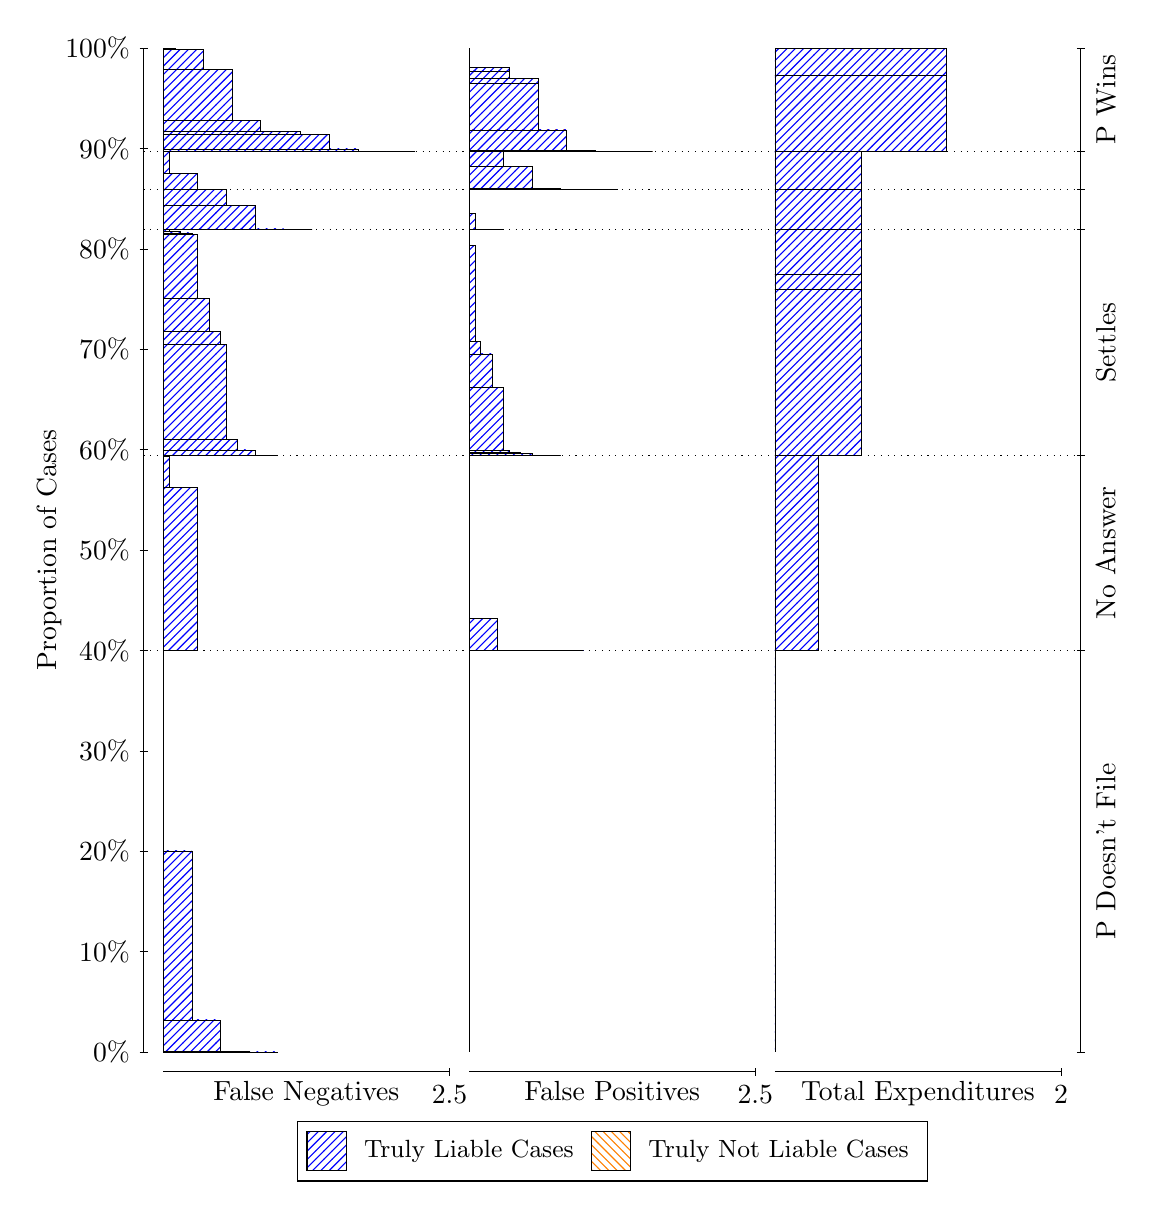
\begin{tikzpicture}
\draw[black, very thin] (1.5,1.75) -- (1.5,14.5);
\node[rotate=90, text=black, anchor=center] at (0.3, 8.125) {Proportion of Cases};
\draw[black, very thin] (1.45,1.75) -- (1.55,1.75);
\node[text=black, anchor=east] at (1.45, 1.75) {0\%};
\draw[black, very thin] (1.45,3.025) -- (1.55,3.025);
\node[text=black, anchor=east] at (1.45, 3.025) {10\%};
\draw[black, very thin] (1.45,4.3) -- (1.55,4.3);
\node[text=black, anchor=east] at (1.45, 4.3) {20\%};
\draw[black, very thin] (1.45,5.575) -- (1.55,5.575);
\node[text=black, anchor=east] at (1.45, 5.575) {30\%};
\draw[black, very thin] (1.45,6.85) -- (1.55,6.85);
\node[text=black, anchor=east] at (1.45, 6.85) {40\%};
\draw[black, very thin] (1.45,8.125) -- (1.55,8.125);
\node[text=black, anchor=east] at (1.45, 8.125) {50\%};
\draw[black, very thin] (1.45,9.4) -- (1.55,9.4);
\node[text=black, anchor=east] at (1.45, 9.4) {60\%};
\draw[black, very thin] (1.45,10.675) -- (1.55,10.675);
\node[text=black, anchor=east] at (1.45, 10.675) {70\%};
\draw[black, very thin] (1.45,11.95) -- (1.55,11.95);
\node[text=black, anchor=east] at (1.45, 11.95) {80\%};
\draw[black, very thin] (1.45,13.225) -- (1.55,13.225);
\node[text=black, anchor=east] at (1.45, 13.225) {90\%};
\draw[black, very thin] (1.45,14.5) -- (1.55,14.5);
\node[text=black, anchor=east] at (1.45, 14.5) {100\%};

\draw[black, very thin] (13.4,1.75) -- (13.4,14.5);
\draw[black, very thin] (13.35,1.75) -- (13.45,1.75);
\node[anchor=west] at (13.35, 1.75) {};
\draw[black, very thin] (13.35,6.8489) -- (13.45,6.8489);
\node[anchor=west] at (13.35, 6.8489) {};
\draw[black, very thin] (13.35,9.322) -- (13.45,9.322);
\node[anchor=west] at (13.35, 9.322) {};
\draw[black, very thin] (13.35,12.194) -- (13.45,12.194);
\node[anchor=west] at (13.35, 12.194) {};
\draw[black, very thin] (13.35,12.706) -- (13.45,12.706);
\node[anchor=west] at (13.35, 12.706) {};
\draw[black, very thin] (13.35,13.191) -- (13.45,13.191);
\node[anchor=west] at (13.35, 13.191) {};
\draw[black, very thin] (13.35,14.5) -- (13.45,14.5);
\node[anchor=west] at (13.35, 14.5) {};

\draw[black, very thin, pattern color=blue, pattern=north east lines] (1.75,1.75) rectangle (3.2033,1.75);
\draw[black, very thin, pattern color=blue, pattern=north east lines] (1.75,1.75) rectangle (2.84,1.7534);
\draw[black, very thin, pattern color=blue, pattern=north east lines] (1.75,1.7534) rectangle (2.4767,2.158);
\draw[black, very thin, pattern color=blue, pattern=north east lines] (1.75,2.158) rectangle (2.1133,4.3029);
\draw[black, very thin, pattern color=orange, pattern=north west lines] (1.75,4.3029) rectangle (1.75,4.3029);
\draw[black, very thin, pattern color=blue, pattern=north east lines] (1.75,4.3029) rectangle (1.75,6.8489);
\draw[black, very thin, pattern color=blue, pattern=north east lines] (1.75,6.8489) rectangle (2.186,8.9179);
\draw[black, very thin, pattern color=blue, pattern=north east lines] (1.75,8.9179) rectangle (1.8227,9.3191);
\draw[black, very thin, pattern color=orange, pattern=north west lines] (1.75,9.3191) rectangle (1.75,9.3191);
\draw[black, very thin, pattern color=blue, pattern=north east lines] (1.75,9.3191) rectangle (1.75,9.322);
\draw[black, very thin, pattern color=blue, pattern=north east lines] (1.75,9.322) rectangle (3.2033,9.322);
\draw[black, very thin, pattern color=blue, pattern=north east lines] (1.75,9.322) rectangle (3.058,9.3223);
\draw[black, very thin, pattern color=blue, pattern=north east lines] (1.75,9.3223) rectangle (2.9127,9.3899);
\draw[black, very thin, pattern color=blue, pattern=north east lines] (1.75,9.3899) rectangle (2.84,9.3976);
\draw[black, very thin, pattern color=blue, pattern=north east lines] (1.75,9.3976) rectangle (2.6947,9.5256);
\draw[black, very thin, pattern color=blue, pattern=north east lines] (1.75,9.5256) rectangle (2.5493,10.74);
\draw[black, very thin, pattern color=blue, pattern=north east lines] (1.75,10.74) rectangle (2.4767,10.9);
\draw[black, very thin, pattern color=blue, pattern=north east lines] (1.75,10.9) rectangle (2.3313,11.325);
\draw[black, very thin, pattern color=blue, pattern=north east lines] (1.75,11.325) rectangle (2.186,12.129);
\draw[black, very thin, pattern color=blue, pattern=north east lines] (1.75,12.129) rectangle (2.1133,12.152);
\draw[black, very thin, pattern color=blue, pattern=north east lines] (1.75,12.152) rectangle (1.968,12.169);
\draw[black, very thin, pattern color=blue, pattern=north east lines] (1.75,12.169) rectangle (1.8227,12.194);
\draw[black, very thin, pattern color=orange, pattern=north west lines] (1.75,12.194) rectangle (1.75,12.194);
\draw[black, very thin, pattern color=blue, pattern=north east lines] (1.75,12.194) rectangle (1.75,12.194);
\draw[black, very thin, pattern color=blue, pattern=north east lines] (1.75,12.194) rectangle (3.6393,12.194);
\draw[black, very thin, pattern color=blue, pattern=north east lines] (1.75,12.194) rectangle (3.276,12.202);
\draw[black, very thin, pattern color=blue, pattern=north east lines] (1.75,12.202) rectangle (2.9127,12.498);
\draw[black, very thin, pattern color=blue, pattern=north east lines] (1.75,12.498) rectangle (2.5493,12.704);
\draw[black, very thin, pattern color=blue, pattern=north east lines] (1.75,12.704) rectangle (2.186,12.706);
\draw[black, very thin, pattern color=orange, pattern=north west lines] (1.75,12.706) rectangle (1.75,12.706);
\draw[black, very thin, pattern color=blue, pattern=north east lines] (1.75,12.706) rectangle (2.186,12.905);
\draw[black, very thin, pattern color=blue, pattern=north east lines] (1.75,12.905) rectangle (1.8227,13.183);
\draw[black, very thin, pattern color=orange, pattern=north west lines] (1.75,13.183) rectangle (1.75,13.183);
\draw[black, very thin, pattern color=blue, pattern=north east lines] (1.75,13.183) rectangle (1.75,13.191);
\draw[black, very thin, pattern color=blue, pattern=north east lines] (1.75,13.191) rectangle (4.9473,13.191);
\draw[black, very thin, pattern color=blue, pattern=north east lines] (1.75,13.191) rectangle (4.584,13.191);
\draw[black, very thin, pattern color=blue, pattern=north east lines] (1.75,13.191) rectangle (4.2207,13.219);
\draw[black, very thin, pattern color=blue, pattern=north east lines] (1.75,13.219) rectangle (3.8573,13.402);
\draw[black, very thin, pattern color=blue, pattern=north east lines] (1.75,13.402) rectangle (3.712,13.402);
\draw[black, very thin, pattern color=blue, pattern=north east lines] (1.75,13.402) rectangle (3.494,13.44);
\draw[black, very thin, pattern color=blue, pattern=north east lines] (1.75,13.44) rectangle (3.3487,13.44);
\draw[black, very thin, pattern color=blue, pattern=north east lines] (1.75,13.44) rectangle (3.1307,13.44);
\draw[black, very thin, pattern color=blue, pattern=north east lines] (1.75,13.44) rectangle (2.9853,13.577);
\draw[black, very thin, pattern color=blue, pattern=north east lines] (1.75,13.577) rectangle (2.7673,13.577);
\draw[black, very thin, pattern color=blue, pattern=north east lines] (1.75,13.577) rectangle (2.622,14.232);
\draw[black, very thin, pattern color=blue, pattern=north east lines] (1.75,14.232) rectangle (2.2587,14.487);
\draw[black, very thin, pattern color=blue, pattern=north east lines] (1.75,14.487) rectangle (1.8953,14.5);
\draw[black, very thin, pattern color=orange, pattern=north west lines] (1.75,14.5) rectangle (1.75,14.5);
\draw[black, very thin, pattern color=blue, pattern=north east lines] (1.75,14.5) rectangle (1.75,14.5);
\draw[black, very thin, pattern color=orange, pattern=north west lines] (5.6333,1.75) rectangle (5.6333,1.75);
\draw[black, very thin, pattern color=blue, pattern=north east lines] (5.6333,1.75) rectangle (5.6333,6.8489);
\draw[black, very thin, pattern color=orange, pattern=north west lines] (5.6333,6.8489) rectangle (7.0867,6.8489);
\draw[black, very thin, pattern color=blue, pattern=north east lines] (5.6333,6.8489) rectangle (7.0867,6.8489);
\draw[black, very thin, pattern color=blue, pattern=north east lines] (5.6333,6.8489) rectangle (6.7233,6.8489);
\draw[black, very thin, pattern color=blue, pattern=north east lines] (5.6333,6.8489) rectangle (6.36,6.8517);
\draw[black, very thin, pattern color=blue, pattern=north east lines] (5.6333,6.8517) rectangle (5.9967,7.2529);
\draw[black, very thin, pattern color=blue, pattern=north east lines] (5.6333,7.2529) rectangle (5.6333,9.322);
\draw[black, very thin, pattern color=orange, pattern=north west lines] (5.6333,9.322) rectangle (6.796,9.322);
\draw[black, very thin, pattern color=blue, pattern=north east lines] (5.6333,9.322) rectangle (6.796,9.322);
\draw[black, very thin, pattern color=orange, pattern=north west lines] (5.6333,9.322) rectangle (6.6507,9.322);
\draw[black, very thin, pattern color=blue, pattern=north east lines] (5.6333,9.322) rectangle (6.6507,9.322);
\draw[black, very thin, pattern color=orange, pattern=north west lines] (5.6333,9.322) rectangle (6.5053,9.322);
\draw[black, very thin, pattern color=blue, pattern=north east lines] (5.6333,9.322) rectangle (6.5053,9.322);
\draw[black, very thin, pattern color=blue, pattern=north east lines] (5.6333,9.322) rectangle (6.4327,9.3471);
\draw[black, very thin, pattern color=blue, pattern=north east lines] (5.6333,9.3471) rectangle (6.2873,9.3641);
\draw[black, very thin, pattern color=blue, pattern=north east lines] (5.6333,9.3641) rectangle (6.142,9.3868);
\draw[black, very thin, pattern color=blue, pattern=north east lines] (5.6333,9.3868) rectangle (6.0693,10.191);
\draw[black, very thin, pattern color=blue, pattern=north east lines] (5.6333,10.191) rectangle (5.924,10.616);
\draw[black, very thin, pattern color=blue, pattern=north east lines] (5.6333,10.616) rectangle (5.7787,10.776);
\draw[black, very thin, pattern color=blue, pattern=north east lines] (5.6333,10.776) rectangle (5.706,11.991);
\draw[black, very thin, pattern color=blue, pattern=north east lines] (5.6333,11.991) rectangle (5.6333,12.194);
\draw[black, very thin, pattern color=orange, pattern=north west lines] (5.6333,12.194) rectangle (6.0693,12.194);
\draw[black, very thin, pattern color=blue, pattern=north east lines] (5.6333,12.194) rectangle (6.0693,12.197);
\draw[black, very thin, pattern color=blue, pattern=north east lines] (5.6333,12.197) rectangle (5.706,12.403);
\draw[black, very thin, pattern color=blue, pattern=north east lines] (5.6333,12.403) rectangle (5.6333,12.706);
\draw[black, very thin, pattern color=orange, pattern=north west lines] (5.6333,12.706) rectangle (7.5227,12.706);
\draw[black, very thin, pattern color=blue, pattern=north east lines] (5.6333,12.706) rectangle (7.5227,12.706);
\draw[black, very thin, pattern color=blue, pattern=north east lines] (5.6333,12.706) rectangle (7.1593,12.706);
\draw[black, very thin, pattern color=blue, pattern=north east lines] (5.6333,12.706) rectangle (6.796,12.714);
\draw[black, very thin, pattern color=blue, pattern=north east lines] (5.6333,12.714) rectangle (6.4327,12.993);
\draw[black, very thin, pattern color=blue, pattern=north east lines] (5.6333,12.993) rectangle (6.0693,13.191);
\draw[black, very thin, pattern color=orange, pattern=north west lines] (5.6333,13.191) rectangle (7.9587,13.191);
\draw[black, very thin, pattern color=blue, pattern=north east lines] (5.6333,13.191) rectangle (7.9587,13.191);
\draw[black, very thin, pattern color=orange, pattern=north west lines] (5.6333,13.191) rectangle (7.5953,13.191);
\draw[black, very thin, pattern color=blue, pattern=north east lines] (5.6333,13.191) rectangle (7.5953,13.191);
\draw[black, very thin, pattern color=orange, pattern=north west lines] (5.6333,13.191) rectangle (7.232,13.191);
\draw[black, very thin, pattern color=blue, pattern=north east lines] (5.6333,13.191) rectangle (7.232,13.204);
\draw[black, very thin, pattern color=blue, pattern=north east lines] (5.6333,13.204) rectangle (6.8687,13.459);
\draw[black, very thin, pattern color=orange, pattern=north west lines] (5.6333,13.459) rectangle (6.8687,13.459);
\draw[black, very thin, pattern color=blue, pattern=north east lines] (5.6333,13.459) rectangle (6.8687,13.459);
\draw[black, very thin, pattern color=blue, pattern=north east lines] (5.6333,13.459) rectangle (6.5053,14.055);
\draw[black, very thin, pattern color=blue, pattern=north east lines] (5.6333,14.055) rectangle (6.5053,14.114);
\draw[black, very thin, pattern color=orange, pattern=north west lines] (5.6333,14.114) rectangle (6.36,14.114);
\draw[black, very thin, pattern color=blue, pattern=north east lines] (5.6333,14.114) rectangle (6.36,14.114);
\draw[black, very thin, pattern color=blue, pattern=north east lines] (5.6333,14.114) rectangle (6.142,14.21);
\draw[black, very thin, pattern color=blue, pattern=north east lines] (5.6333,14.21) rectangle (6.142,14.251);
\draw[black, very thin, pattern color=orange, pattern=north west lines] (5.6333,14.251) rectangle (5.9967,14.251);
\draw[black, very thin, pattern color=blue, pattern=north east lines] (5.6333,14.251) rectangle (5.9967,14.251);
\draw[black, very thin, pattern color=blue, pattern=north east lines] (5.6333,14.251) rectangle (5.7787,14.251);
\draw[black, very thin, pattern color=blue, pattern=north east lines] (5.6333,14.251) rectangle (5.7787,14.251);
\draw[black, very thin, pattern color=orange, pattern=north west lines] (5.6333,14.251) rectangle (5.6333,14.251);
\draw[black, very thin, pattern color=blue, pattern=north east lines] (5.6333,14.251) rectangle (5.6333,14.5);
\draw[black, very thin, pattern color=orange, pattern=north west lines] (9.5167,1.75) rectangle (9.5167,1.75);
\draw[black, very thin, pattern color=blue, pattern=north east lines] (9.5167,1.75) rectangle (9.5167,6.8489);
\draw[black, very thin, pattern color=orange, pattern=north west lines] (9.5167,6.8489) rectangle (10.062,6.8489);
\draw[black, very thin, pattern color=blue, pattern=north east lines] (9.5167,6.8489) rectangle (10.062,9.322);
\draw[black, very thin, pattern color=orange, pattern=north west lines] (9.5167,9.322) rectangle (10.607,9.322);
\draw[black, very thin, pattern color=blue, pattern=north east lines] (9.5167,9.322) rectangle (10.607,11.434);
\draw[black, very thin, pattern color=orange, pattern=north west lines] (9.5167,11.434) rectangle (10.607,11.434);
\draw[black, very thin, pattern color=blue, pattern=north east lines] (9.5167,11.434) rectangle (10.607,11.624);
\draw[black, very thin, pattern color=orange, pattern=north west lines] (9.5167,11.624) rectangle (10.607,11.624);
\draw[black, very thin, pattern color=blue, pattern=north east lines] (9.5167,11.624) rectangle (10.607,12.194);
\draw[black, very thin, pattern color=orange, pattern=north west lines] (9.5167,12.194) rectangle (10.607,12.194);
\draw[black, very thin, pattern color=blue, pattern=north east lines] (9.5167,12.194) rectangle (10.607,12.706);
\draw[black, very thin, pattern color=orange, pattern=north west lines] (9.5167,12.706) rectangle (10.607,12.706);
\draw[black, very thin, pattern color=blue, pattern=north east lines] (9.5167,12.706) rectangle (10.607,13.191);
\draw[black, very thin, pattern color=orange, pattern=north west lines] (9.5167,13.191) rectangle (11.697,13.191);
\draw[black, very thin, pattern color=blue, pattern=north east lines] (9.5167,13.191) rectangle (11.697,14.151);
\draw[black, very thin, pattern color=orange, pattern=north west lines] (9.5167,14.151) rectangle (11.697,14.151);
\draw[black, very thin, pattern color=blue, pattern=north east lines] (9.5167,14.151) rectangle (11.697,14.5);
\draw[black, dotted] (1.5,6.8489) -- (13.4,6.8489);
\draw[black, dotted] (1.5,9.322) -- (13.4,9.322);
\draw[black, dotted] (1.5,12.194) -- (13.4,12.194);
\draw[black, dotted] (1.5,12.706) -- (13.4,12.706);
\draw[black, dotted] (1.5,13.191) -- (13.4,13.191);
\draw[black, very thin] (1.75,1.5) -- (5.3833,1.5);
\node[text=black, anchor=north] at (3.5667, 1.5) {False Negatives};
\draw[black, very thin] (5.3833,1.45) -- (5.3833,1.55);
\node[text=black, anchor=north] at (5.3833, 1.45) {2.5};

\draw[black, very thin] (5.6333,1.5) -- (9.2667,1.5);
\node[text=black, anchor=north] at (7.45, 1.5) {False Positives};
\draw[black, very thin] (9.2667,1.45) -- (9.2667,1.55);
\node[text=black, anchor=north] at (9.2667, 1.45) {2.5};

\draw[black, very thin] (9.5167,1.5) -- (13.15,1.5);
\node[text=black, anchor=north] at (11.333, 1.5) {Total Expenditures};
\draw[black, very thin] (13.15,1.45) -- (13.15,1.55);
\node[text=black, anchor=north] at (13.15, 1.45) {2};

\node[text=black, centered, rotate=90] at (13.72, 4.2994) {P Doesn't File};
\node[text=black, centered, rotate=90] at (13.72, 8.0854) {No Answer};
\node[text=black, centered, rotate=90] at (13.72, 10.758) {Settles};


\node[text=black, centered, rotate=90] at (13.72, 13.846) {P Wins};

\draw (7.449999999999999,1.5) node[draw=none] (baseCoordinate) {};
\begin{scope}[align=center]
        \matrix[scale=0.5, draw=black, below=0.5cm of baseCoordinate, nodes={draw}, column sep=0.1cm]{
            \node[rectangle, draw, minimum width=0.5cm, minimum height=0.5cm, pattern color=blue, pattern=north east lines] {}; &
            \node[draw=none, font=\small, text=black] (B) {Truly Liable Cases}; &
            \node[rectangle, draw, minimum width=0.5cm, minimum height=0.5cm, pattern color=orange, pattern=north west lines] {}; &
            \node[draw=none, font=\small, text=black] (B) {Truly Not Liable Cases}; \\
            };
\end{scope}

\end{tikzpicture}
\end{document}